	\chapter{Das Strahlungstransportproblem}
	\label{sec:radiative_transfer}
	
	Das Verhalten von Licht lässt sich (nach heutigem wissenschaftlichen Stand) durch die {\em Quantenelektrodynamik}\footnote{siehe z.B. \citet{Feynman:1990p11684}} in allen Details vollständig beschreiben. Es beinhaltet solche Phänomene wie Dispersion, Brechung, Interferenz, Photon--Photon--Interaktion, etc. Diese Effekte sind häufig dann am bedeutendsten, wenn die Ausmaße der betrachteten Objekte von der Größenordnung der Wellenlänge des Lichtes sind. Auf der anderen Seite beschreibt die {\em geometrische Optik} die rein makroskopische lineare Ausbreitung großer Mengen von Photonen, ohne obengenannte Wellen--Phänomene zu berücksichtigen.
	
	Beim Strahlungstransportproblem (STP) sind wir an einer {\em phänomenologischen} Beschreibung interessiert. Das heißt wir wollen die Effekte des Lichts modellieren, die in typischen Anwendungen durch optische Instrumente (Auge, Teleskope mit Photoplatten/CCD--Chips) gemessen werden können. Dies bedeutet, dass wir hauptsächlich eine geometrische Beschreibung des Lichts in Form eines Teilchentransportproblems ansetzen aber relevante quantenmechanische Effekte wie Photonen--Streuung in erster Ordnung lokal mitberücksichtigen (z.B. in Form einer Streuphasenfunktion).
	
	Die folgende Darstellung und Herleitung orientiert sich an \citep{Arvo:1993p9035}.
	
	\section{Das Strahlungstransportproblem als Teilchentransportproblem}
	Um Strahlungstransport als Teilchentransportproblem behandeln zu können, müssen folgende Bedingungen erfüllt sein:
	\begin{itemize}
		\item{Die Teilchen müssen so klein und zahlreich sein, dass ihre statistische Verteilung als kontinuierlich angesehen werden kann}
		\item{Zu jedem Zeitpunkt lässt sich ein Teilchen komplett durch seinen Positionsvektor, Geschwindigkeitsvektor und eventuelle interne Zustände (wie Polarisation, Frequenz, Ladung, Spin, etc.) charakterisieren}
	\end{itemize}
	Diese Annahmen sind für Photonen und die uns interessierenden räumlichen Entfernungen erfüllt.
	Darüber hinausgehend machen wir im Rahmen dieser Arbeit folgende Annahmen:
	\begin{itemize}
		\item{Die Materialeigenschaften ändern sich bei Variation des Ortes in der Größenordnung der Wellenlänge nur wenig}
		\item{Das Strahlungsintensitätsfeld ist stationär (d.h. innerhalb der typischen Zeiten, die ein Photon braucht um das Simulationsgebiet zu durchqueren, können die Materialeigenschaften als statisch angenommen werden)}
		\item{Photonen werden ausschließlich elastisch gestreut}
		\item{der Raum wird als euklidisch angenommen (d.h. es werden keine relativistischen Effekte berücksichtigt)}
	\end{itemize}
	Die Annahme ausschließlich elastischer Streuvorgänge erlaubt es uns, das Strahlungstransportproblem für jede Wellenlänge getrennt zu betrachten, da Photonen bei elastischer Streuung ihre Wellenlänge nicht ändern und somit den Strahlungstransport in anderen Wellenlängen nicht beeinflussen. Daher behandeln wir im Folgenden nur das monochromatische Strahlungstransportproblem, in dem Wissen, dass der polychromatische Fall immer als eine Reihe von monochromatischen Problemen behandelt werden kann. Aufgrund der monochromatischen (und damit monoenergetischen) Annahme ist der Teilchenimpuls und somit die Teilchengeschwindigkeit konstant. Daher reicht es zur vollständigen Beschreibung eines Teilchenzustandes aus, wenn wir nur die Position $\location{r}$ (entsprechend drei Freiheitsgraden) und die Bewegungsrichtung $\omega$ (entsprechend zwei Freiheitsgraden) des Teilchens angeben. Wir können nun ein Teilchen als Punkt des zugehörigen fünf--dimensionalen Phasenraums $\mathbb{R}^3 \times \mathcal{S}^2$ identifizieren, wobei $\mathbb{R}^3$ den euklidischen Raum und $\mathcal{S}^2$ die Einheitskugel im $\mathbb{R}^3$ meint.
	
	Um die statistische Verteilung unserer Teilchen im Phasenraum zu jedem Zeitpunkt spezifizieren zu können führen wir die Phasenraumdichte $n$ ein, sodass $$n(\location{r},\omega,t)\,d\location{r}\,d\omega$$ der Anzahl Teilchen entspricht, die sich zum Zeitpunkt $t$ in einem infinitesimalen Volumen $d\location{r}$ um $\location{r} \in \mathbb{R}^3$ befinden und sich in eine Richtung bewegen, die innerhalb eines infinitesimalen Raumwinkels $d\omega$ um $\omega \in \mathcal{S}^2$ liegt. Damit hat $n$ die Einheit $\text{m}^{-3}\text{sr}^{-1}$. Die Phasenraumdichte trifft keine Aussage über Materialeigenschaften oder innere Zustände der Teilchen, wie Masse oder Frequenz, sondern beschreibt lediglich deren Anzahldichte im Phasenraum. Physikalisch relevante Größen (wie z.B. die Intensität) führen wir später (in Abschnitt \ref{subsec:strahlungsgroessen}) auf die Phasenraumdichte zurück. An dieser Stelle erlaubt die abstraktere Natur von $n$ aber eine klarere Darstellung der wesentlichen Verhaltensweisen der Teilchen. Von der Phasenraumdichte lassen sich alle für uns interessanten Größen prinzipiell ableiten, für die folgende Herleitung ist es aber praktischer wenn wir uns die Rate der Teilchen, die eine imaginäre Fläche durchqueren, anschauen.
	
	Sei $d\location{A}$ eine infinitesimales Flächenelement, $\omega$ die Flächennormale von $d\location{A}$ und $d\omega$ ein infinitesimales Raumwinkelelement, das $\omega$ beinhaltet (siehe Abb.~(\ref{fig:phasespacefluxsurface})). Betrachten wir nun die Teilchen, welche die Fläche $d\location{A}$ in einem Zeitraum $dt$ mit Bewegungsrichtung innerhalb $d\omega$ passieren. Alle diese Teilchen liegen im Volumen $d\location{A}\,ds$ wobei $ds=v\,dt$ und $v$ die Geschwindigkeit der Teilchen ist. Nehmen wir an, dass $\location{r}$ innerhalb diese Volumens liegt, ist die Anzahl der Teilchen $$n(\location{r},\omega,t)\,d\location{A}\,ds\,d\omega.$$ Wenn wir stattdessen aber nach der Rate fragen, mit der die Teilchen $d\location{A}$ passieren, erhalten wir den Phasenraumfluß $$\phi(\location{r},\omega,t):=v\,n(\location{r},\omega,t)$$ mit der Einheit $[\phi]=\text{m}^{-2}\text{sr}^{-1}s^{-1}$. Die Teilchenanzahl in $d\location{A}\,ds$ mit dem Phasenraumfluss ausgedrückt ist $$\phi(\location{r},\omega,t)\,d\location{A}\,d\omega\,dt.$$
	\begin{figure}
		\centering
		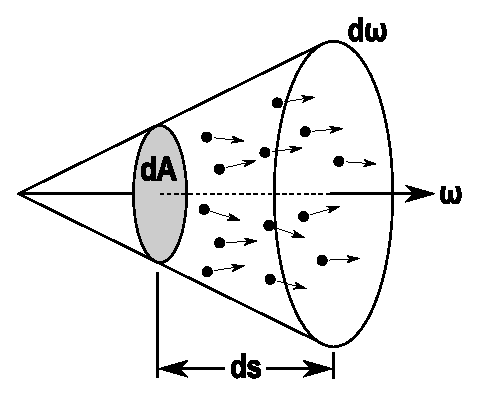
\includegraphics[height=0.3\textheight]{phasespacefluxsurface.eps}
		\caption{Teilchen, die das infinitesimale Flächenelement $d\location{A}$ durchqueren und sich in eine Richtung innerhalb des infinitesimalen Raumwinkelelements $d\omega$ um die Flächennormale $\omega$ von $d\location{A}$ bewegen.}
		\label{fig:phasespacefluxsurface}
	\end{figure}
	Der Phasenraumfluss ist ebenso wie die Phasenraumdichte eine fundamentale Größe, aus der wir alle anderen interessanten Größen ableiten können. Im Folgenden werden wir uns aber meist auf den Phasenraumfluss beziehen.
		
	Unser Ziel ist es nun eine Bilanzgleichung für die Teilchen in einem beliebigen Teil $V \times \Omega$ des Phasenraums (siehe Abb.~(\ref{fig:phasespacevolume})) aufzustellen. Dabei ist $V \subset \mathbb{R}^3$ ein Teilvolumen des $\mathbb{R}^3$ und $\Omega \subset \mathcal{S}^2$ ein beliebiger Raumwinkel aus der Einheitskugel $\mathcal{S}^2$. Dazu betrachten wir erst einmal die möglichen Gründe, die zu einer Veränderung der Teilchenzahl in unserem betrachteten Phasenraumvolumen $V \times \Omega$ führen können.
	\begin{figure}
		\centering
		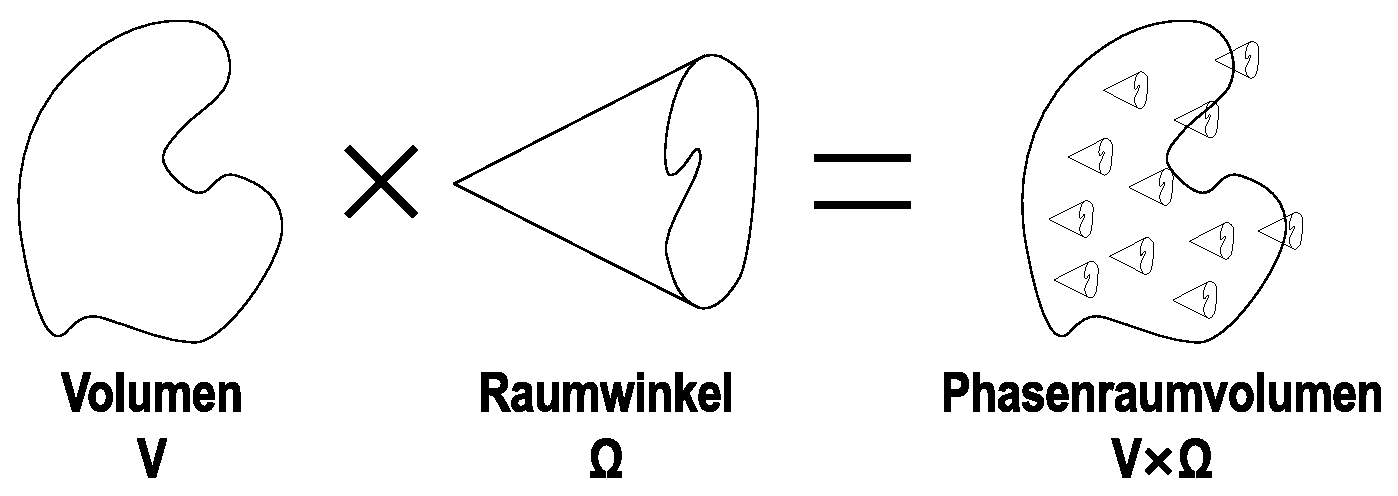
\includegraphics[width=0.8\textwidth]{phasespacevolume.eps}
		\caption{Darstellung einer Teilmenge $V \times \Omega$ des Phasenraums. Sie repräsentiert alle Teilchen, die sich innerhalb des Volumens $V$ befinden und sich in eine Richtung innerhalb von $\Omega$ bewegen.}
		\label{fig:phasespacevolume}
	\end{figure}

	Zur {\em Emission} zählt jeder Prozess, der neue Teilchen erzeugt. Dies kann durch verschiedene physikalische Prozesse wie z.B. chemische Reaktionen, thermische Emission oder Kernfusion begründet sein. Emission innerhalb von $V$ in eine Richtung innerhalb von $\Omega$ verändert also die Teilchenbilanz, da sie eine Quelle für Teilchen darstellt. Nach der Emission bewegen sich die Teilchen in unserem Modell gradlinig mit konstanter Geschwindigkeit bis sie eine instantane Kollision mit dem Medium erfahren. Bewegt sich ein Teilchen bei seiner gradlinigen Bewegung in das Volumen $V$ hinein oder aus ihm heraus und bewegt es sich dabei in eine Richtung innerhalb von $\Omega$, so ändert dies ebenfalls unsere Teilchenbilanz. In diesem Fall sprechen wir von {\em Durchströmen}. Findet als letzte Möglichkeit eine {\em Kollision} des Teilchens mit dem Medium innerhalb von $V$ statt, kann das Teilchen entweder absorbiert oder gestreut werden. Wird es absorbiert wirkt dies als Teilchensenke. Wird es gestreut, dann kann es, je nachdem in welche Richtung es sich vor und nach der Kollision bewegt hat, entweder keinen Einfluss auf die Teilchenbilanz haben (Bewegungsrichtung vor und nach der Kollision entweder innerhalb oder außerhalb von $\Omega$), es kann herausgestreut werden (Bewegungsrichtung vor der Kollision innerhalb und nach der Kollision ausserhalb von $\Omega$) oder aber hineingestreut werden (Bewegungsrichtung vor der Kollision ausserhalb und nach der Kollision innerhalb von $\Omega$) werden.
	
	Um die einzelnen Beiträge dieser Prozesse zur Teilchenbilanz quantitativ zu erfassen führen wir die Teilchenzahl $$N(t):=\int_\Omega \int_V n(\location{r},\omega,t)\,d\location{r}\,d\omega$$ ein. Sie gibt an wieviele Teilchen sich zum Zeitpunkt $t$ im Phasenraumvolumen $V \times \Omega$ befinden. Durch die eben beschriebenen Prozesse ändert sich $N(t)$ normalerweise mit der Zeit. Ist die Zeit, die ein Teilchen benötigt das betrachtete System zu durchqueren, klein gegenüber der typischen Zeitskala, nach der sich das System bedeutend verändert hat, können wir annehmen, dass sich die Teilchenzahl für jedes Phasenraumvolumen im dynamischen Gleichgewicht befindet, d.h. dass zwar ständig Teilchen aus dem Phasenraumvolumen hinein- und hinausströmen, erzeugt, absorbiert und gestreut werden, aber sich alle Prozesse in der Bilanz die Waage halten, $N(t)$ also stationär ist:$$\frac{dN(t)}{dt}=0\qquad\left[\frac{1}{\text{s}}\right].$$ Teilen wir diese änderung von $N$ mit der Zeit auf die verschiedenen obengenannten Prozesse auf, sind wir bei der Grundlage einer Bilanzgleichung angelangt:$$\begin{bmatrix}\text{änderung}\\ \text{durch}\\ \text{Emission}\end{bmatrix}+\begin{bmatrix}\text{änderung}\\ \text{durch}\\ \text{Durchströmung}\end{bmatrix}+\begin{bmatrix}\text{änderung}\\ \text{durch}\\ \text{Kollisionen}\end{bmatrix}=0.$$ Wir leiten nun für jeden dieser Ausdrücke einen Formelausdruck her.
	Die änderung aufgrund von Emission nennen wir $$\mathbf{E}=\int_\Omega \int_V q(\location{r},\omega)\,d\location{r}\,d\omega\qquad\left[\frac{1}{\text{s}}\right],$$ wobei wir die Phasenraumquellfunktion $q$ (mit Einheit $\text{m}^{-3}\text{sr}^{-1}\text{s}^{-1}$) eingeführt haben, die für jeden Ort $\location{r}$ und jede Raumrichtung $\omega$ die Anzahl erzeugter Teilchen pro Sekunde, Einheitsvolumen und Einheitsraumwinkel angibt. Hinein- und herausströmende Teilchen erzeugen eine Teilchenrate
	$$\mathbf{S}=\int_\Omega \int_{\partial V} \phi(\location{s},\omega)(\omega \cdot d\location{s})d\omega,$$
	die wir durch Integrieren über $\partial V$ (die Oberfläche von V) erhalten. Hierbei steht $\location{s}$ für ein infinitesimales als Vektor repräsentiertes Flächenelement, dessen Richtung die Flächennormale, und dessen Länge seine Fläche repräsentiert. Das Skalarprodukt zwischen Bewegungsrichtung $\omega$ und Flächennormalen sorgt für das richtige Vorzeichen, wobei ein positiver Wert Teilchenverlust bedeutet.
	Der letzte Beitrag $\mathbf{C}$ trägt den Kollisionen Rechnung. Da Teilchen nur mit dem Medium, nicht aber untereinander interagieren, muss die Kollisionsrate unabhängig von $\phi$ sein. Wir unterteilen $\mathbf{C}$ in einen Absorptionsteil $\mathbf{C}_\text{abs}$ und einen Streuanteil $\mathbf{C}_\text{sca}$. Wir nehmen an, dass die Wahrscheinlichkeit, dass ein Teilchen aufgrund von Absorption verschwindet proportional zur zurückgelegten Distanz im Medium, nicht aber von der Bewegungsrichtung durch das Medium ist (was gleichbedeutend mit der Annahme eines isotropen Mediums ist). Die Proportionalitätskonstante am Ort $\location{r}$ nennen wir den (Volumen-)Absorptionsquerschnitt $\kappa(\location{r})$ ($[\kappa]=\frac{1}{\text{m}}=\frac{m^2}{m^3}$). Die zugehörige Teilchenrate ist
	$$\mathbf{C}_\text{abs}=\int_\Omega \int_V \kappa(\location{r})\phi(\location{r},\omega)\,d\location{r}\,d\omega.$$
	Die genauen Mechanismen der Streuung können durch Mie--Theorie oder Quantenmechanik behandelt werden. In unserem Teilchentransport repräsentieren wir diese Streumodelle durch die Streuphasenfunktion $k(\location{r},\omega,\omega')$ und den Volumenstreuquerschnitt $\sigma(\location{r})$. Dabei gibt $k(\location{r},\omega,\omega')$ bei Streuung eines aus Richtung $\omega$ kommenden Teilchens am Ort $\location{r}$ die Wahrscheinlichkeit pro Einheitsraumwinkel an, nach $\omega'$ gestreut zu werden. Da ein gestreutes Teilchen irgendwohin gestreut wird, gilt für $k$ die Normierungsbedingung
	\begin{equation}\label{eq:k_norm_req}
	  \int_{\mathcal{S}^2} k(\location{r},\omega,\omega')\,d\omega'=1.
	\end{equation}
	Außerdem ist $k$ symmetrisch bezüglich der Vertauschung der Bewegungsrichtungen vor und nach der Streuung:
	$$k(\location{r},\omega,\omega')=k(\location{r},\omega',\omega)\quad \forall\:\omega,\omega'\in\mathcal{S}^2.$$
	Beide Bedingungen werden z.B. durch die isotrope Streuphasenfunktion $$k_\text{iso}(\location{r},\omega,\omega')=\frac{1}{4\pi}$$ erfüllt.
	Wie bei der Absorption, nehmen wir an, dass die Wahrscheinlichkeit eines Teilchens gestreut zu werden von der durch das Medium zurückgelegten Distanz, nicht aber von der Bewegungsrichtung abhängt. Wir teilen $\mathbf{C}_\text{sca}$ weiter auf, in einen Teil
	$$\mathbf{C}_\text{out}=\int_\Omega \int_V \int_{\mathcal{S}^2} \sigma{(\location{r})}k(\location{r},\omega,\omega')\phi(\location{r},\omega)\,d\omega'\,d\location{r}\,d\omega,$$
	der herausgestreute Teilchen berücksichtigt, sowie einen Teil
	$$\mathbf{C}_\text{in}=\int_\Omega \int_V \int_{\mathcal{S}^2} \sigma{(\location{r})}k(\location{r},\omega',\omega)\phi(\location{r},\omega')\,d\omega'\,d\location{r}\,d\omega$$
	entsprechend für hineingestreute Teilchen. Dabei sollte erwähnt werden, dass sowohl $\mathbf{C}_\text{out}$ als auch $\mathbf{C}_\text{in}$ Teilchen berücksichtigen, deren Richtung vor und nach der Streuung in $\Omega$ liegt, was weder einem Zuwachs noch einem Verlust an Teilchen entspricht. Da für unsere Bilanz aber immer nur die Differenz von $\mathbf{C}_\text{out}$ und $\mathbf{C}_\text{in}$ betrachtet wird, hebt sich dieser Teil wieder heraus. Alternativ könnten wir auch über $\mathcal{S}^2 \setminus \Omega$ integrieren, was zu einer komplizierteren Rechnung, aber zu keinem anderen Endergebnis führen würde. Fügen wir die Einzelterme zusammen und ordnen nach Zuwächsen und Verlusten sieht unsere Bilanzgleichung für die Teilchenraten in $V \times \Omega$ wie folgt aus:
	$$\underbrace{\mathbf{S}+\mathbf{C}_\text{abs}+\mathbf{C}_\text{out}}_\text{Verluste}=\underbrace{\mathbf{E}+\mathbf{C}_\text{in}}_\text{Zuwächse}$$
	Es fällt bei der Betrachtung der Formeln für die einzelnen Terme auf, dass alle Terme bis auf $\mathbf{S}$ Volumenintegrale über $V$ enthalten. $\mathbf{S}$ enthält stattdessen ein Oberflächenintegral über $\partial V$. Mithilfe des Gauss'schen Satzes drücken wir das Oberflächenintegral über $\partial V$ durch ein Volumenintegral über $V$ aus und erhalten
	$$\mathbf{S}=\int_\Omega \int_V \omega \cdot (\nabla\phi)(\location{r},\omega)\,d\location{r}\,d\omega,$$
	wobei wir $\nabla \cdot(\omega\phi)=\omega\cdot(\nabla\phi)$ benutzt haben.
	
	In unserer Bilanzgleichung treten jetzt nur noch Volumenintegrale über unser Phasenraumvolumen $V \times \Omega$ auf. Da $V$ und $\Omega$ beliebig gewählt waren, muß die Bilanzgleichung überall und in alle Richtungen lokale Gültigkeit haben:
	\begin{multline*}
	  \omega\cdot\nabla\phi(\location{r},\omega)+\kappa(\location{r})\phi(\location{r},\omega)+\int_{\mathcal{S}^2}\sigma(\location{r})k(\location{r},\omega,\omega')\phi(\location{r},\omega)d\omega' \\
	  =q(\location{r},\omega)+\int_{\mathcal{S}^2}\sigma(\location{r})k(\location{r},\omega',\omega)\phi(\location{r},\omega')d\omega'
	\end{multline*}
	Da beim $\mathbf{C}_\text{out}$--Integral $\sigma$ und $\phi$ nicht von der Integrationsvariable abhängen und das verbleibende Integral aufgrund der Normierungsbedingung (\ref{eq:k_norm_req}) gleich eins ist vereinfacht sich unsere Bilanzgleichung schlussendlich zu
	\begin{equation}\label{eq:particle_balance_equation}
	  \omega\cdot\nabla\phi(\location{r},\omega)+\left(\kappa(\location{r})+\sigma(\location{r})\right)\phi(\location{r},\omega)
	  =q(\location{r},\omega)+\sigma(\location{r})\int_{\mathcal{S}^2}k(\location{r},\omega',\omega)\phi(\location{r},\omega')d\omega'
	\end{equation}
	Die Bilanzgleichung hat die Gestalt einer Integro--Differentialgleichung in $\phi$.
	Im folgenden Abschnitt stellen wir den Bezug zwischen unseren abstrakten Teilchentransportgrößen und physikalischen Strahlungsgrößen her.

	\section{Phänomenologische Strahlungsgrößen}\label{subsec:strahlungsgroessen}
	Im vorigen Abschnitt haben wir das Strahlungstransportproblem bewusst auf ein Teilchentransportproblem mit abstrakten Teilchen statt Photonen reduziert um einerseits eine klarere Herleitung zu ermöglichen und um andererseits die Verwandtschaft zu anderen Transportproblemen (wie z.B. Neutronentransport) offensichtlich zu machen. Um nun den Anschluss zu radiometrischen Strahlungsgrößen zu bekommen, ersetzen wir unsere abstrakten Teilchen wieder durch Photonen. Photonen haben zwei Eigenschaften die wir berücksichtigen müssen. Sie bewegen sich konstant mit Lichtgeschwindigkeit, d.h. wir können die vorher gebrauchte allgemeine Teilchengeschwindigkeit $v$ gleich $\text{c}$ setzten. Außerdem besitzt jedes Photon eine Energie, die durch seine Frequenz $\nu$ mit 
	$$E=h\nu \qquad[J]$$
	bestimmt ist. Dabei bezeichnet $h$ das Planck'sche Wirkungsquantum.
	Jeder Frequenz $\nu$ können wir ein monochromatisches Transportproblem zuordnen, dessen Lösung in Form eines Phasenraumflusses $\phi_\nu$ die Photonenfrequenz als Index trägt.
	Die {\em spezifische Intensität} $I_\nu(\location{r},\omega)$ erhalten wir nun aus dem Phasenraumfluss bzw. der Phasenraumdichte gemäß
	\begin{align}\label{eq:intensity_def}
		I_\nu(\location{r},\omega)d\nu & = h\nu\,\phi_\nu(\location{r},\omega)\\
		                       & = c h\nu\,n_\nu(\location{r},\omega) \qquad \left[\frac{\text{W}}{\text{m}^2\text{sr}}\right] \nonumber
	\end{align}
	Sie gibt an, wieviel Joule am Ort $\location{r}$ pro Sekunde durch eine Einheitsfläche mit Flächennormale $\omega$ pro Einheitsraumwinkel in Richtung $\omega$ und pro Frequenzintervall durch Photonen mit Frequenz $\nu$ transportiert wird:
	$$dE_\nu=I_\nu(\location{r},\omega) dA\,dt\,d\omega\,d\nu.$$
	Wir führen außerdem die {\em spezifische Emissivität} $\varepsilon_\nu$ ein. Wir erhalten Sie aus der Phasenraumquellfunktion $q_\nu$ durch
	\begin{equation}\label{eq:emissivity_def}
		\varepsilon_\nu(\location{r},\omega)d\nu = h\nu\,q_\nu(\location{r},\omega) \qquad \left[\frac{\text{W}}{\text{m}^3\text{sr}}\right].
	\end{equation}
	
	Multiplizieren wir unsere abstrakte Transportgleichung (\ref{eq:particle_balance_equation}) mit $h\nu$ und benutzen wir die Beziehungen (\ref{eq:intensity_def},\ref{eq:emissivity_def}) erhalten wir mit
	\begin{equation}\label{eq:stg_diff}
	  \omega\cdot\nabla I_\nu(\location{r},\omega)+\left(\kappa_\nu(\location{r})+\sigma_\nu(\location{r})\right)I_\nu(\location{r},\omega)
	  =\varepsilon_\nu(\location{r},\omega)+\sigma_\nu(\location{r})\int_{\mathcal{S}^2}k_\nu(\location{r},\omega',\omega)I_\nu(\location{r},\omega')d\omega'
	\end{equation}
	die {\em Strahlungstransportgleichung in differentieller Form}. Sie stellt eine Integro--Differentialgleichung für $I_\nu$ auf unserem 5--dimensionalen Phasenraum $\mathbb{R}^3 \times \mathcal{S}^2$ dar und kann für jede Frequenz $\nu$ getrennt gelöst werden. Sie gibt für jede Kombination aus Ort $\location{r}$ und Photonen--Ausbreitungsrichtung $\omega$ das lokal zu erfüllende Gleichgewicht aus Verlusten (linke Seite) und Zuwächsen (rechte Seite) an.
	
	Wir fassen die Verluste aufgrund von Absorption und Streuung durch den {\em Vo\-lu\-men\-ex\-tink\-ti\-ons\-quer\-schnitt}
	$$\xi_\nu(\location{r}):=\kappa_\nu(\location{r})+\sigma_\nu(\location{r}) \qquad\left[\frac{1}{m}\right]$$
	zusammen, wodurch wir (\ref{eq:stg_diff}) auch als
	\begin{equation}\label{eq:stg_diff2}
	  \omega\cdot\nabla I_\nu(\location{r},\omega)+\xi_\nu(\location{r})I_\nu(\location{r},\omega)
	  =\varepsilon_\nu(\location{r},\omega)+\sigma_\nu(\location{r})\int_{\mathcal{S}^2}k_\nu(\location{r},\omega',\omega)I_\nu(\location{r},\omega')d\omega'
	\end{equation}
	schreiben können.
	Außerdem definieren wir die dimensionslose {\em optische Tiefe}
	\begin{equation*}
		\tau_\nu(\location{r}_1,\location{r}_2):=\int_{s=0}^{||\location{r}_2-\location{r}_1||} \xi_\nu(\location{r}_1+s(\location{r}_2 - \location{r}_1))\,ds,
	\end{equation*}
	die ein Maß für die Undurchsichtigkeit des Mediums bei der Frequenz $\nu$ zwischen zwei Orten $\location{r}_1$ und $\location{r}_2$ ist. Nehmen wir uns Gleichung (\ref{eq:stg_diff2}), betrachten nur die Verluste (indem wir die rechte Seite zu Null setzen) und wählen eine beliebige Richtung $\omega$, gelangen wir zur gewöhnlichen Differentialgleichung
	$$I_\nu'(s)+\xi_\nu(s)I_\nu(s)=0,$$
	die durch
	\begin{equation}
		I_\nu(s)=I_\nu(0)\:\text{exp}\left(-\int_{s'=0}^s \xi_\nu(s')\right)=I_\nu(0)\:\text{exp}\left(-\tau_\nu(0,s)\right)
		\label{eq:exponentialdecay}
	\end{equation}
	gelöst wird. Die Lösung zeigt, dass die optische Tiefe zu einer exponentiellen Abschwächung der Intensität führt. Nach der Definition der verschiedenen phänomenologischen Strahlungsgrößen schauen wir uns nun an, wie ihre Messung aufgefasst und mathematisch definiert werden kann.
	
	
	\section{Die Messgleichung}\label{sec:measurement_equation}
	Mit dem Strahlungsintensitätsfeld, dass aus der Gesamtheit aller spezifischen Intensitäten $I_\nu$ besteht, meinen wir die Funktion
	$$I:\mathbb{R}_+\times\mathbb{R}^3\times\mathcal{S}^2\to\mathbb{R}_+\;,\qquad (\nu,\location{r},\omega)\mapsto I_\nu(\location{r},\omega),$$
	die vom 6--dimensionalen Raum aller Photonenfrequenzen, Orte und Raumrichtungen auf die dort herrschende spezifische Intensität abbildet.
	
	Funktionen dieser Art bilden einen Skalarproduktraum. Das Null--Element ist die konstant auf Null abbildende Funktion. Zwei Funktionen lassen sich punktweise addieren und ergeben so eine neue Funktion, die auch nach $\mathbb{R}_{\geq 0}$ abbildet. Das Skalarprodukt zwischen zwei Funktionen $f$ und $g$ ist schließlich mit
	$$\langle f,g\rangle=\int_{\mathbb{R}_+} \int_{\mathbb{R}^3} \int_{\mathcal{S}^2} f(\nu,\location{r},\omega)g(\nu,\location{r},\omega)\,d\omega\,d\location{r}\,d\nu$$
	gegeben.
	
	Mit diesem funktionalanalytischen Handwerkszeug definieren wir eine Messung als das Skalarprodukt zwischen unserem Strahlungsintensitätsfeld $I$ und einer {\em Sensitivitätsfunktion} $W$, welche die Stärke der Gewichtung angibt, mit der die spezifische Intensität der Frequenz $\nu$ am Ort $\location{r}$ in Richtung $\omega$ in den Messwert eingeht. Die entsprechende Formel
	\begin{equation}\label{eq:messgleichung}
		M^{(i)}:=\langle W^{(i)},I\rangle=\int_{\mathbb{R}_+} \int_{\mathbb{R}^3} \int_{\mathcal{S}^2} W^{(i)}(\nu,\location{r},\omega)I_\nu(\location{r},\omega)\,d\omega\,d\location{r}\,d\nu
	\end{equation}
	nennen wir {\em Messgleichung} (für den $i$--ten Sensor). Für monochromatische Messungen führen wir zusätzlich noch 
	\begin{equation}\label{eq:messgleichung_mono}
		M_\nu^{(i)}:=\langle W_\nu^{(i)},I_\nu\rangle=\int_{\mathbb{R}^3} \int_{\mathcal{S}^2} W_\nu^{(i)}(\location{r},\omega)I_\nu(\location{r},\omega)\,d\omega\,d\location{r}
	\end{equation}
	ein, womit wir (\ref{eq:messgleichung}) auch als
	\begin{equation}\label{eq:messgleichung_frommonos}
		M^{(i)}=\int_{\mathbb{R}_+} M_\nu^{(i)}\,d\nu
	\end{equation}
	schreiben können.
	Die Tatsache, dass wir die Sensitivitätsfunktion nicht näher spezifizieren, erlaubt uns die größtmögliche Freiheit beim kreieren virtueller Sensoren. Beispielsweise könnte $W$ nur in einem kleinen Volumen und einem kleinen Raumwinkel, aber bei allen Frequenzen, nichtverschwindend sein, und so einen virtuellen Sensor zur Messung der Gesamt--Intensität an einem bestimmten Ort in eine bestimmte Richtung repräsentieren. Ebenso kann durch gleichstarke Gewichtung aller Raumrichtungen die mittlere Intensität gemessen werden.
	
	Was hier vielleicht als ein nur theoretisch interessantes Konstrukt ohne praktischen Nutzen erscheint, erweist sich später insbesondere in Verbindung mit Monte--Carlo--Sampling als ein gleichzeitig vielseitiges und effizientes Werkzeug.	
	
	
	\section{übersicht etablierter Lösungsverfahren}
	TODO: übersicht benutzter Lösungsverfahren, Meilensteine (wann zum ersten mal Polarisation gerechnet?, Warum etablieren sich MC-Verfahren so spät?, etc...)
		
	\chapter{Pfadintegralformulierung der Strahlungstransportgleichung}\label{chapter:path_radiative_transfer}
	In diesem Abschnitt leiten wir eine alternative mathematische Formulierung der Strahlungstransportgleichung einerseits und ihrer Lösung (genau genommen, Messungen der Lösung im Sinne von (\ref{eq:messgleichung})) andererseits her. Dies führt uns durch die verschiedenen auf das Problem eingenommenen Blickwinkel zu einem besseren Verständnis von Strahlungstransport und gibt uns darüber hinaus einen neuen Ansatzpunkt zur effizienten Lösung des Strahlungstransportproblems.
	
	Die Idee zu dieser Formulierung kommt aus der Dissertation von \citet{Veach:1997p9136}, wird aber schon in \citep{Arvo:1995p9257} vorgestellt. Beide Dissertationen behandeln allerdings nur den Strahlungstransport zwischen Oberflächen. In der Arbeit von \citet{Pauly:2000p5705} wird dies auf partizipierende Medien ausgedehnt. Aus \citep{Arvo:1993p9035} stammt außerdem die Herleitung der integralen Form der Strahlungstransportgleichung.
	
	
	\section{Strahlungstransportgleichung in integraler Form}
	In differentieller Form nimmt die Strahlungstransportgleichung, wie wir in Abschnitt (\ref{subsec:strahlungsgroessen}) gesehen haben, folgende Gestalt an:
		\begin{equation}
			\omega \cdot \nabla I(\location{r},\omega)+\overbrace{\left(\kappa(\location{r})+\sigma(\location{r})\right)}^{=:\xi(\location{r})}I(\location{r},\omega)=\varepsilon(\location{r},\omega)+\sigma(\location{r}) \int_{\mathcal{S}^2} k(\location{r},\omega',\omega)I(\location{r},\omega') d\omega'.
			\label{eq:diff.STG}
		\end{equation}
	Für diesen und die folgenden Abschnitte lassen wir dabei den Index $\nu$ aus übersichtsgründen weg, womit gemeint ist, dass wir stellvertretend für alle Frequenzen ein einzelnes monochromatisches Strahlungstransportproblem einer beliebigen Frequenz nehmen. Wenn wir zum polychromatischen Fall zurückkehren führen wir die Indizes wieder ein.
	
	Schreiben wir das Skalarprodukt zwischen $\omega$ und dem $\nabla$--Operator als Richtungsableitung
	\newcommand{\dds}{\frac{\text{d}}{\text{d}s}}
	\newcommand{\ddszero}{\left. \dds \right|_{s=0}}
	\begin{equation*}
		\omega \cdot \nabla I(\location{r},\omega)
		=  \ddszero I(\location{r}+s\,\omega,\omega)
		=  -\ddszero I(\location{r}-s\,\omega,\omega)
	\end{equation*}
	können wir (\ref{eq:diff.STG}) als
	\begin{multline}
		\dds I(\location{r}-s\,\omega,\omega) - \xi(\location{r}-s\,\omega)I(\location{r}-s\,\omega,\omega) = \\-\varepsilon(\location{r}-s\,\omega,\omega) -\sigma(\location{r}-s\,\omega) \int_{\mathcal{S}^2} k(\location{r}-s\,\omega,\omega',\omega)I(\location{r}-s\,\omega,\omega') \text{d}\omega'
		\label{eq:diff.STGtranslated}
	\end{multline}
	umschreiben. Dabei haben wir die Beschränkung $s=0$ fallengelassen, was die Korrektheit der Umformung aber nicht ändert. Mit den Abkürzungen
	\begin{align*}
		{\hat I}(s)&:=I(\location{r}-s\,\omega,\omega) \\
		Q(\location{r},\omega)&:= \varepsilon(\location{r},\omega)+\sigma(\location{r}) \int_{\mathcal{S}^2} k(\location{r},\omega',\omega)I(\location{r},\omega') d\omega' \\
		{\hat Q}(s)&:=Q(\location{r}-s\,\omega,\omega)\\
		{\hat \xi}(s)&:=\xi(\location{r}-s\,\omega) \\
		{\hat \tau}(s)&:= \int_{s'=0}^{s} {\hat \xi}(s') \text{d}s'
	\end{align*}
	wird aus (\ref{eq:diff.STGtranslated})
	\begin{equation}
		\dds {\hat I}(s) - {\hat \xi}(s){\hat I}(s)= -{\hat Q}(s) \qquad |\cdot e^{-{\hat \tau}(s)}.
		\label{eq:diff.STGhatted}
	\end{equation}
	Gleichung (\ref{eq:diff.STGhatted}) ist eine gewöhnliche Differentialgleichung die sich mit
	\begin{align}
		(\ref{eq:diff.STGhatted})\Leftrightarrow\qquad \dds \left(e^{-{\hat \tau}(s)} {\hat I}(s)\right)&= -e^{-{\hat \tau}(s)} {\hat Q}(s) \qquad | \int_{s'=0}^s (\cdot)\text{d}s' \nonumber \\
		\Leftrightarrow\qquad e^{-{\hat \tau}(s)} {\hat I}(s) - {\hat I}(0) &= -\int_{s'=0}^s e^{-{\hat \tau}(s')} {\hat Q}(s') \text{d}s' \nonumber \\
		\Leftrightarrow\qquad {\hat I}(0) &= e^{-{\hat \tau}(s)} {\hat I}(s) + \int_{s'=0}^s e^{-{\hat \tau}(s')} {\hat Q}(s') \text{d}s' \label{eq:diff.STGpreintegral}
	\end{align}
	leicht nach ${\hat I}(0)$ auflösen lässt. Obwohl ${\hat Q}(s)$ lokal die Intensität $I$ über alle Raumrichtungen integriert, dürfen wir für die Lösung von (\ref{eq:diff.STGhatted}) $Q$ als unabhängig von $I$ behandeln, da die Schnittmenge zwischen der Geraden im Raum, auf der wir die Differentialgleichung lösen, und der Menge aller Raumrichtungen $\mathcal{S}^2$ bei der Integration über alle Raumrichtungen eine Nullmenge ist und somit für physikalisch relevante Strahlungsintensitätsfelder (d.h. solche, die hinreichend stetig/beschränkt bzw. keine Delta--Distribution sind) keinen Beitrag zum Integral leistet.
	Setzen wir in (\ref{eq:diff.STGpreintegral}) für die Abkürzungen wieder die ursprünglichen Ausdrücke ein, erhalten wir die {\em Strahlungstransportgleichung in integraler Form}:
	\begin{multline}
		I(\location{r},\omega) = e^{-\tau(\location{r},\location{r}-s\,\omega)} {\hat I}(\location{r},\location{r}-s\,\omega) + \int_{s'=0}^\infty e^{-\tau(\location{r},\location{r}-s\,\omega)} \;\cdot \\
		\quad\cdot\left( \varepsilon(\location{r}-s'\,\omega,\omega) + \sigma(\location{r}-s'\,\omega)
		\left[ \int_{\mathcal{S}^2} k(\location{r}-s'\,\omega,\omega',\omega)I(\location{r}-s'\,\omega,\omega') \text{d}\omega'\right] \right) \text{d}s'
		\label{eq:int.STG}
	\end{multline}
	Nehmen wir nun als Randbedingungen an, dass in unendlich großer Entfernung keine Lichtquellen existieren, d.h. $\forall \omega \in \mathcal{S}^2 : I(\location{r}=-\infty\cdot\omega,\omega)=0$, dann vereinfacht sich (\ref{eq:int.STG}) zu
	\begin{multline}
		I(\location{r},\omega) = \int_{s'=0}^\infty e^{-\tau(\location{r},\location{r}-s\,\omega)} \;\cdot \\
		\quad\cdot\left( \varepsilon(\location{r}-s'\,\omega,\omega) + \sigma(\location{r}-s'\,\omega)
		\left[ \int_{\mathcal{S}^2} k(\location{r}-s'\,\omega,\omega',\omega)I(\location{r}-s'\,\omega,\omega') \text{d}\omega'\right] \right) \text{d}s'
		\label{eq:int.STGdarkbg}
	\end{multline}


	\section{Strahlungstransportgleichung in Operator--Form}
	Schauen wir uns die einzelnen Teile der Gleichung (\ref{eq:int.STGdarkbg}) genauer an.
	Der innere Teil von (\ref{eq:int.STGdarkbg}) in eckigen Klammern summiert an einem festen Ort ($\location{r}-s'\,\omega$), mit der Streuphasenfunktion $k$ gewichtet, die einfallenden Intensitäten auf, die in Richtung $\omega$ gestreut werden. Anschließend skaliert der Volumenstreuquerschnitt die aufintegrierte Intensität entsprechend dem lokal vorhandenen Medium und gibt dabei dem Ausdruck die Einheit einer Emissivität.
	Der restliche äußere Teil der Gleichung addiert die eben gewonnene Emissivität durch Einstreuung zu der lokal durch Ausstrahlung erzeugten Emissivität an jedem Punkt auf einer Geraden hinter dem Punkt $\location{r}$ und summiert die mit einem der optischen Tiefe entsprechenden Abschwächungsfaktor gewichteten, in Richtung $\omega$ zeigenden, Emissivitäten, entlang der Geraden zur Gesamtintensität am Ort $\location{r}$ in Richtung $\omega$ auf.
	Der Gesamtausdruck lässt sich durch Einführung zweier neuer Operatoren
	\begin{align*}
		\left(\mathbf{G}\varepsilon\right)(\location{r},\omega)&:=\int_{s'=0}^\infty e^{-\tau(\location{r}-s' \omega,\location{r})}\varepsilon(\location{r}-s' \omega,\omega) ds' \\
		\left(\mathbf{K}I\right)(\location{r},\omega)&:=\sigma(\location{r})\int_{S^2} k(\location{r},\omega',\omega) I(\location{r},\omega') d\omega'
	\end{align*}
	\begin{equation*}
		\mathbf{G} : \varepsilon(\location{r},\omega) \mapsto I(\location{r},\omega) , \qquad
		\mathbf{K} : I(\location{r},\omega) \mapsto \varepsilon(\location{r},\omega)
	\end{equation*}
	in elementarere Prozesse aufteilen. Wir nennen $\mathbf{G}$ den sogenannten {\em Fortpflanzungs--Operator} und $\mathbf{K}$ den {\em Streu--Operator}. Beides sind Integraloperatoren auf dem Raum der Funktionen $f : \mathbb{R}^3 \times \mathcal{S}^2 \to \mathbb{R}_+$, die vom Teilchen--Phasenraum auf die positiven reellen Zahlen abbilden. Beide haben komplementäre Lokalitäten. Während $\mathbf{K}$ lokal im Ort über alle Raumrichtungen integriert, ist $\mathbf{G}$ lokal in der Raumrichtung und integriert über alle Orte entlang einer Geraden im Raum. Dabei bildet $\mathbf{K}$ von einem Strahlungsintensitätsfeld auf ein Emissivitätsfeld ab. Bei $\mathbf{G}$ ist es umgekehrt, es macht aus einem Emissivitätsfeld wieder ein Strahlungsintensitätsfeld.
	Mit diesen neuen Operatoren wird aus Gleichung (\ref{eq:int.STGdarkbg}) die {\em Operatorform der Strahlungstransportgleichung}
	\begin{equation}
		I=\mathbf{G}(\varepsilon + \mathbf{K}I),
		\label{eq:op.STG}
	\end{equation}
	die wir nach $I$ auflösen können:
	\begin{align}
		(\ref{eq:op.STG}) \Leftrightarrow I&=\mathbf{G}\varepsilon + \mathbf{GK}I \nonumber \\
		\Leftrightarrow (\mathbf{1}-\mathbf{GK})I &= \mathbf{G}\varepsilon \nonumber \\
		\Leftrightarrow I &= (\mathbf{1}-\mathbf{GK})^{-1}\mathbf{G}\varepsilon \label{eq:op.STGinvert} \\
		\Leftrightarrow I &= \sum_{k=0}^\infty (\mathbf{GK})^k \mathbf{G}\varepsilon \label{eq:op.STGneumann} \\
		&=\mathbf{G}\varepsilon + \mathbf{GKG}\varepsilon + \mathbf{GKGKG}\varepsilon + \hdots \label{eq:op.STGneumann.explicit} \\
		\Leftrightarrow I &=\sum_{k=0}^\infty \mathbf{G} (\mathbf{KG})^k \varepsilon \label{eq:op.STGkg}
	\end{align}
	Damit ist das Strahlungstransportproblem formal gelöst! Dabei haben wir den auftretenden invertierten Operator (\ref{eq:op.STGinvert}) durch eine Neumann--Reihe (\ref{eq:op.STGneumann}) ersetzt. Dies ist dann zulässig wenn die Operatornorm des Operators $\mathbf{GK}$ kleiner als eins ist und damit sichergestellt ist, dass die Neumann--Reihe konvergiert. Für alle praktisch relevanten Probleme ist dies der Fall \citep[siehe][Theorem 12 und 13]{Arvo:1995p9257}. Physikalisch lässt sich das Gleichgewichts--Strahlungsintensitätsfeld als Summe aus Intensitätsfeldern verstehen, die durch Photonen mit unterschiedlich vielen Streuereignissen auf ihrem Weg von der Emission aus einer Lichtquelle bis zu ihrer Messung mit einem Messinstrument entstanden sind (wie in Schritt (\ref{eq:op.STGneumann.explicit}) deutlich wird). Dabei müssen Pfade jeder möglichen Länge (sprich Anzahl an Streuereignissen) berücksichtigt werden. Zwischen Emission und Messung wechseln sich dabei Fortpflanzung $\mathbf{G}$ und Streuung $\mathbf{K}$ ab. Im letzen Schritt (\ref{eq:op.STGkg}) haben wir $\mathbf{G}$ nach links ausgeklammert um den $\mathbf{KG}$--Operator herauszustellen.
	
	
	\section{KG--Operator in Volumenform}
	Schauen wir uns den $\mathbf{KG}$--Operator genauer an. Nachdem $\mathbf{KG}$ ein Emissivitätsfeld durch Fortpflanzung zu einem Intensitätsfeld aufintegriert hat, wird dieses durch die anschliessende Streuung erneut auf ein Emissivitätsfeld abgebildet:
	\begin{equation*}
		\mathbf{KG} : \varepsilon(\location{r},\omega) \mapsto \varepsilon(\location{r},\omega)
	\end{equation*}

	Setzen wir die Definitionen der Operatoren ein und fassen die Integrale zusammen:
	\begin{align*}
		\left(\mathbf{KG}\varepsilon\right)(\location{r},\omega)&=\sigma(\location{r}) \int_{\mathcal{S}^2} k(\location{r},\omega',\omega)\left[\int_{s'=0}^\infty e^{-\tau(\location{r}-s' \omega',\location{r})}\varepsilon(\location{r}-s' \omega',\omega') \text{d}s'\right] \text{d}\omega' \\
		&=\sigma(\location{r}) \int_{\mathcal{S}^2} \int_{s'=0}^\infty k(\location{r},\omega',\omega) e^{-\tau(\location{r}-s' \omega',\location{r})}\varepsilon(\location{r}-s' \omega',\omega') \underbrace{\text{d}s' \text{d}\omega'}_{=\frac{\text{d}\location{r}'}{s'^2}} \\
		&=\sigma(\location{r}) \int_{\mathbb{R}^3} k(\location{r},\omega',\omega) \frac{e^{-\tau(\location{r}',\location{r})}}{\|\location{r}-\location{r}'\|^2}\varepsilon(\location{r}',\omega') \,\text{d}\location{r}'
	\end{align*}
	Da wir durch Kombination der Integration über alle Raumrichtungen $\omega'$ und alle Entfernungen $s'$ den gesamten Raum abdecken, können wir die beiden Integrale zugunsten eines Volumenintegrals über den gesamten Raum und einen geometrischen Verdünnungsfaktor tauschen. Mit dem Ziel, später alle Integrationen zu Volumenintegralen zusammenzufassen, schreiben wir den $\mathbf{KG}$--Operator so um, dass alle expliziten Angaben von Entfernungen und Raumrichtungen durch eine raumpunktorientierte Notation ersetzt werden:
	\begin{multline}
		\left(\mathbf{KG}\varepsilon\right)(\location{r}_i \rightarrow\location{r}_{i+1})=\\
		\sigma(\location{r}_i) \int_{\mathbb{R}^3} k(\location{r}_{i-1}\rightarrow\location{r}_i\rightarrow\location{r}_{i+1})\frac{e^{-\tau(\location{r}_{i-1},\location{r}_i)}}{\|\location{r}_i-\location{r}_{i-1}\|^2}\varepsilon(\location{r}_{i-1} \rightarrow\location{r}_i)d\location{r}_{i-1}
		\label{eq:KGvolume_intermediate}
	\end{multline}
	Wir führen zusätzlich noch die Abkürzung
	\begin{align*}
		\scatter{i}\;&:=\sigma(\location{r}_i)k(\location{r}_{i-1}\rightarrow\location{r}_i\rightarrow\location{r}_{i+1})\\
			&=\sigma(\location{r}_i)k(\location{r}_i,\normalized{\location{r}_i-\location{r}_{i-1}},\normalized{\location{r}_{i+1}-\location{r}_i})
	\end{align*}
	ein, so dass wir (\ref{eq:KGvolume_intermediate}) zusammen mit den in Abschnitt \ref{subsec:nomenklatur} eingeführten Schreibweisen noch kompakter als
	\begin{equation}
		\left(\mathbf{KG}\varepsilon\right)_{(i,i+1)}=\int_{\mathbb{R}^3} \scatter{i}\frac{e^{-\tau_{(i-1,i)}}}{d_{(i-1,i)}^2}\varepsilon_{(i-1,i)}d\location{r}_{i-1}.
		\label{eq:KGvolume}
	\end{equation}
	schreiben können.


	\section{Pfadintegrallösung der Strahlungstransportgleichung}
	Wir setzen die Neumann--Reihen--Lösung (\ref{eq:op.STGkg}) in die monochromatische Meßgleichung (\ref{eq:messgleichung_mono}) ein und erhalten
	\begin{align}
		M_\nu&=\int_{\mathbb{R}^3}\int_{\mathcal{S}^2}W_\nu(\location{r},\omega) \left(\sum_{k=0}^\infty \mathbf{G} (\mathbf{KG})^k \varepsilon_\nu\right)(\location{r},\omega) \,\text{d}\omega \,\text{d}\location{r} \nonumber \\
		&=\sum_{k=0}^\infty \int_{\mathbb{R}^3}\int_{\mathcal{S}^2}W_\nu(\location{r},\omega) \left(\mathbf{G} (\mathbf{KG})^k \varepsilon_\nu\right)(\location{r},\omega) \,\text{d}\omega \,\text{d}\location{r} \nonumber \\
		&=\sum_{k=0}^\infty \int_{\mathbb{R}^3}\int_{\mathcal{S}^2}W_\nu(\location{r},\omega) \int_{s'=0}^\infty e^{-\tau_\nu(\location{r}-s' \omega,\location{r})} \left((\mathbf{KG})^k \varepsilon_\nu\right)(\location{r},\omega) \underbrace{\text{d}s' \,\text{d}\omega}_{=\frac{\text{d}\location{r}'}{s'^2}} \,\text{d}\location{r} \nonumber \\
		&=\sum_{k=0}^\infty \int_{\mathbb{R}^3}\int_{\mathbb{R}^3}W_\nu(\location{r}'\rightarrow\location{r}) \frac{e^{-\tau_\nu(\location{r}',\location{r})}}{\|\location{r}'-\location{r}\|^2} \left((\mathbf{KG})^k \varepsilon_\nu\right)(\location{r}'\rightarrow\location{r}) \,\text{d}\location{r}' \,\text{d}\location{r}.
		\label{eq:STGprepathsolution}
	\end{align}
	Durch rekursives Einsetzen von (\ref{eq:KGvolume}) in (\ref{eq:STGprepathsolution}) und Neuanordnung der Terme erhalten wir dann als Ergebnis einer monochromatischen Messung:
	\begin{equation}
		M_\nu=\sum_{k=0}^\infty \underbrace{\idotsint}_{(k+2)\text{--mal}}\varepsilon_{\nu,(0,1)}\left[\prod_{i=1}^k\frac{e^{-\tau_{\nu,(i-1,i)}}}{d_{(i-1,i)}^2}\scatter{i}\right]\frac{e^{-\tau_{\nu,(k,k+1)}}}{d_{(k,k+1)}^2} W_{\nu,(k,k+1)} \;\text{d}\location{r}_0 \dotsm \text{d}\location{r}_{k+1} .
		\label{eq:STGpathsolution}
	\end{equation}
	Das Ergebnis ist eine Summe aus reinen $(k+2)$--fachen Volumenintegralen über den ganzen Raum, wobei über den möglichen Start- und Endpunkt sowie die $k$ Streupunkte innerhalb des Photonenpfades integriert wird.
	Anschaulich müssen wir also die Beiträge von Pfaden jeder Anzahl an Streupunkten und jeder möglichen Anordnung von Emissions-, Streu- und Mess\-orten aufsummieren. Dies wird vielleicht klarer, wenn wir die ersten Terme der Summe explizit ausformulieren:
	\begin{align*}
		M_\nu&=\iint_{(\mathbb{R}^3)^2}\varepsilon_{\nu,(0,1)}\frac{e^{-\tau_{\nu,(0,1)}}}{d_{(0,1)}^2} W_{\nu,(0,1)} \;\text{d}\location{r}_0\text{d}\location{r}_1 \\
		&+\iiint_{(\mathbb{R}^3)^3}\varepsilon_{\nu,(0,1)}\frac{e^{-\tau_{\nu,(0,1)}}}{d_{(0,1)}^2}\scatter{1}\frac{e^{-\tau_{\nu,(1,2)}}}{d_{(1,2)}^2} W_{\nu,(1,2)} \;\text{d}\location{r}_0\text{d}\location{r}_1\text{d}\location{r}_2 \\
		&+\iiiint_{(\mathbb{R}^3)^4}\varepsilon_{\nu,(0,1)}\frac{e^{-\tau_{\nu,(0,1)}}}{d_{(0,1)}^2}\scatter{1}\frac{e^{-\tau_{\nu,(1,2)}}}{d_{(1,2)}^2}\scatter{2}\frac{e^{-\tau_{\nu,(2,3)}}}{d_{(2,3)}^2} W_{\nu,(2,3)} \;\text{d}\location{r}_0\text{d}\location{r}_1\text{d}\location{r}_2\text{d}\location{r}_3 \\
		&+\hdots
	\end{align*}
	Diese Form der Lösung des Strahlungstransportproblems hat mehrere Vorteile:
	\begin{itemize}
		\item{Die Lösung besitzt eine anschauliche Interpretation}
		\item{Die Lösung ist explizit, es muss keine implizite Integro--Differentialgleichung wie (\ref{eq:stg_diff}) gelöst werden}
		\item{Die Lösung ist ein reines Integrationsproblem und somit ein gutes Gegenstück zu hochdimensionalen Monte--Carlo--Integrations--Verfahren, wie wir in Abschnitt \ref{subsec:integrationsproblem_comparison} sehen werden}
	\end{itemize}
	Das polychromatische Messergebnis ergibt sich nun einfach durch Einsetzen von (\ref{eq:STGpathsolution}) in (\ref{eq:messgleichung_frommonos}).


	\section{Elimination der Neumann--Reihe}\label{sec:neumann_elimination}
	Unsere Darstellung der Lösung (\ref{eq:STGpathsolution}) des Strahlungstransportproblems besteht bisher aus einer unendlichen Summe von Integralen, was eine direkte Folge der Aufspaltung des Lösungsoperators aus (\ref{eq:op.STGinvert}) in seine Neumann--Reihe (\ref{eq:op.STGneumann}) ist. In dieser Form sind die Pfade in Klassen gleicher Länge (d.h. Anzahl an Streupunkten) eingeteilt, was die mathematische Behandlung vereinfacht, da die Fälle verschiedener Länge getrennt voneinander behandelt werden können. Gleichzeitig verleitet diese Darstellung jedoch dazu zu glauben, es wäre sinnvoll oder läge in der Natur der Sache, die Pfade unterschiedlicher Länge getrennt voneinander zu behandeln. Tatsächlich gibt es aber keinen physikalischen Grund dafür, vielmehr wäre es auch mathematisch hilfreich die Lösung als ein einziges Integral über den Raum aller Pfade darzustellen, da wir es dann formal mit nur noch einem Integrationsproblem zu tun hätten und nicht mehr mit unendlich vielen.
	
	Daher führen wir nun \citet[][8.2]{Veach:1997p9136} folgend, die Menge aller Pfade sowie ein passendes Integrationsmaß ein, um unsere Lösung (\ref{eq:STGpathsolution}) als Einzelintegral darstellen zu können. Sei dazu $\Omega_{\nu,k}$ die Menge aller Pfade der Frequenz $\nu$ und der Länge $k$, d.h. Pfade der Form
	$${\overline x}=\location{r}_0\location{r}_1\cdots\location{r}_k\location{r}_{k+1},$$
	mit $k\in\{0,1,2,\dots\}$ und $\location{r}_i \in \mathbb{R}^3$ für alle $i$. Wir definieren mittels
	$$\mu_k(D)=\int_D d\nu d\location{r}_0\cdots d\location{r}_{k+1}$$
	ein Maß für Pfade der Länge $k$, wobei $D\subset\Omega_k$ eine Teilmenge von Pfaden dieser Länge repräsentiert und $d\location{r}_i$ das geometrische Volumenmaß sowie $d\nu$ das Integrationsmaß über die positiven reellen Zahlen darstellt. Die Menge aller Pfade ist die Vereinigung
	$$\Omega=\bigcup_{k=0}^\infty \Omega_k$$
	der Mengen von Pfaden verschiedener Längen. Daß Maß für die Integration von beliebigen Teilmengen des Pfadraumes $D\subset\Omega$ ist nun durch
	$$\mu(D)=\sum_{k=0}^\infty \mu_k(D\cap\Omega_k)$$
	gegeben, d.h. das Maß für $D$ ist einfach die Summe der Maße von Pfaden aus $D$ entsprechender Länge. Benennen wir nun noch den pfadlängen- und frequenzabhängigen Integranden aus (\ref{eq:STGpathsolution})
	\begin{equation}
		f({\overline x}_\nu)=f_\nu(\location{r}_0\location{r}_1\cdots\location{r}_k\location{r}_{k+1})=\varepsilon_{\nu,(0,1)}\left[\prod_{i=1}^k\frac{e^{-\tau_{\nu,(i-1,i)}}}{d_{(i-1,i)}^2}\scatter{i}\right]\frac{e^{-\tau_{\nu,(k,k+1)}}}{d_{(k,k+1)}^2} W_{\nu,(k,k+1)}
		\label{eq:mcf}
	\end{equation}
	als {\em Messbeitragsfunktion} $f$, dann können wir nun die polychromatische Messung (\ref{eq:messgleichung}) einfach als
	\begin{equation}
		M=\int_\Omega f({\overline x})d\mu({\overline x})
		\label{eq:unified_measurementintegral}
	\end{equation}
	schreiben. Es ist in dieser Form leichter einzusehen, dass wir die Pfade nicht nach ihrer Länge zusammengefasst behandeln müssen, um anschließend die (unendlich vielen) Ergebnisse aufzusummieren, sondern stattdessen Pfade in beliebiger Weise zur Integration zusammenfassen dürfen. Dies ist insbesondere für die Monte--Carlo--Integration wichtig, da unsere ganze Theorie sich dort auf die Lösung eines Einzelintegrals beschränken wird und wir dadurch dort nahtlos mit der Lösung von Messintegralen der Form (\ref{eq:unified_measurementintegral}) anknüpfen können.
